\chapter{Funcionamento da Aplicação UMeR}
\section{Menu Inicial}
Esta é  uma aplicação com uma interface para o utilizador muito simples, foi pensada
de maneira a que o utilizador pudesse tirar o maior proveito da mesma, com comandos simples, tendo em conta que todos os menus funcionam à base de opções por números.
Quando um utilizador executa a aplicação o primeiro menu a que está sujeito é o
seguinte:

\begin{figure}[htpb]
\centering
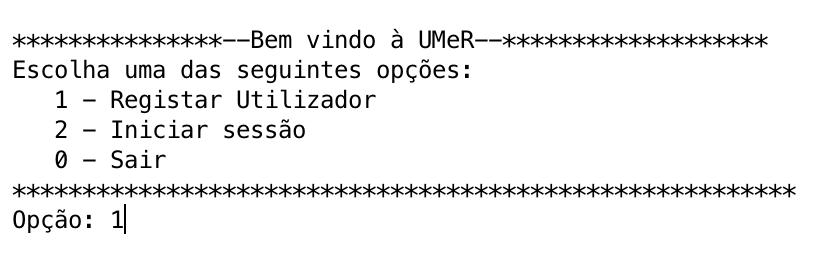
\includegraphics[scale=0.6]{imagem/menuInicial}
\caption{Menu Inicial  }
\label{p3:fig:p2_paginicial}
\end{figure}

\subsection{Registo}

O utilizador consoante o seu tipo poderá efetuar um registo na aplicação. Será apresentado o seguinte menu para o registo de atores no sistema: 

\begin{figure}[htpb]
	\centering
	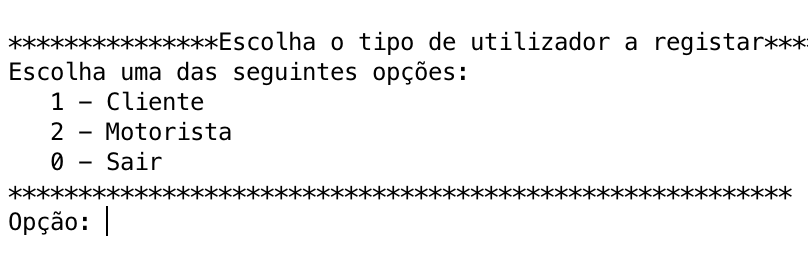
\includegraphics[scale=0.6]{imagem/escolhaTipoAtor}
	\caption{Menu de Registo na Aplicação }
	\label{p3:fig:p2_escolhaTipoAtor}
\end{figure}
Os dados pedidos no ato de registo quer de clientes ou motoristas é o mesmo, no entanto serão guardados de acordo com o tipo inicialmente escolhido. 
\newline

\noindent\begin{minipage}[b]{.4\textwidth}
	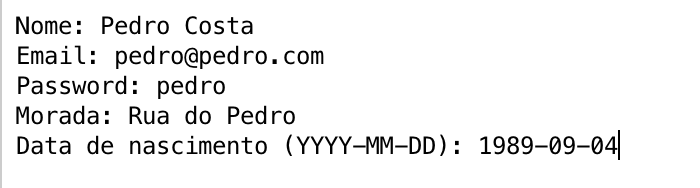
\includegraphics[scale=0.6]{imagem/exemploregistomotorista}
	\small{Exemplo de registo de um motorista}
\end{minipage} 
\hfill
\begin{minipage}[b]{.4\textwidth}
	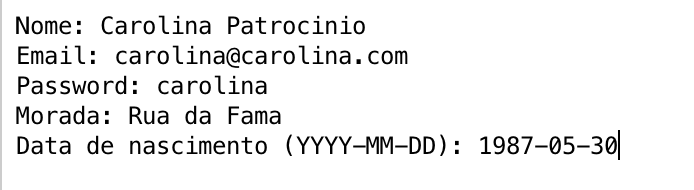
\includegraphics[scale=0.6]{imagem/exemploderegistocliente}
	\small{Exemplo de registo de um cliente}
\end{minipage}
\hfill

\subsection{Iniciar Sessão }
\subsubsection{Cliente}
O Cliente tem à sua disposição várias funcionalidades tais como: Soliciar uma viagem; Visualizar o histórico de viagens; Classificar viagens e ainda Ver e Editar dados pessoais. 
\begin{figure}[htpb]
	\centering
	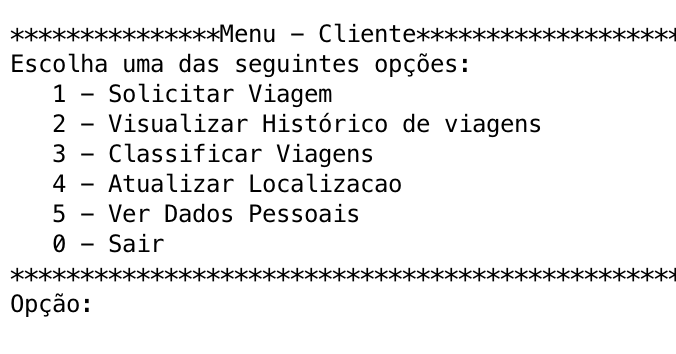
\includegraphics[scale=0.7]{imagem/menuCliente}
	\caption{Menu de Cliente }
	\label{p3:fig:p3_menuCliente}
\end{figure}

Ao escolher "Solicitar Viagem" será pedido ao Cliente para introduzir as Coordenadas de destino. Após a inserção das Coordenadas é pedido ao Cliente para escolher se quer o táxi que se encontra mais próximo dele ou se prefere escolher um táxi que permite fila de espera se estiver ocupado. 

\noindent\begin{minipage}[b]{.5\textwidth}
	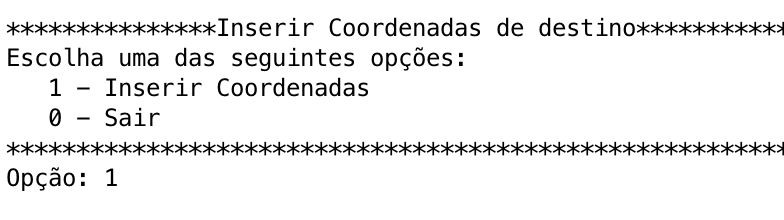
\includegraphics[scale=0.55]{imagem/inserirDestino}
	\small{Menu para inserir as coordenadas}
\end{minipage} 
\hfill
\begin{minipage}[b]{.5\textwidth}
	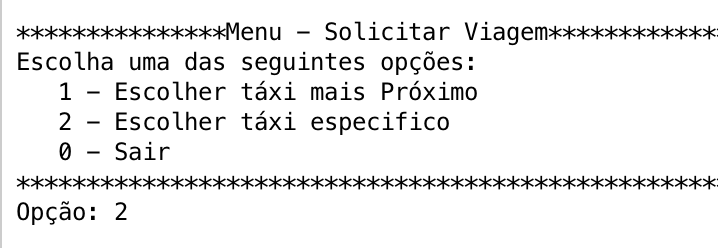
\includegraphics[scale=0.6]{imagem/coorInseridas}
	\small{Menu após a inserção de coordenadas: Escolha de táxi}
\end{minipage}
\hfill


O Cliente após escolher a opção 1, é-lhe apresentado um menu com os dados do táxi que se encontra mais perto da localização do cliente. De seguida é dada a opção de aceitar fazer a viagem ou não. 
\begin{figure}[htpb]
	\centering
	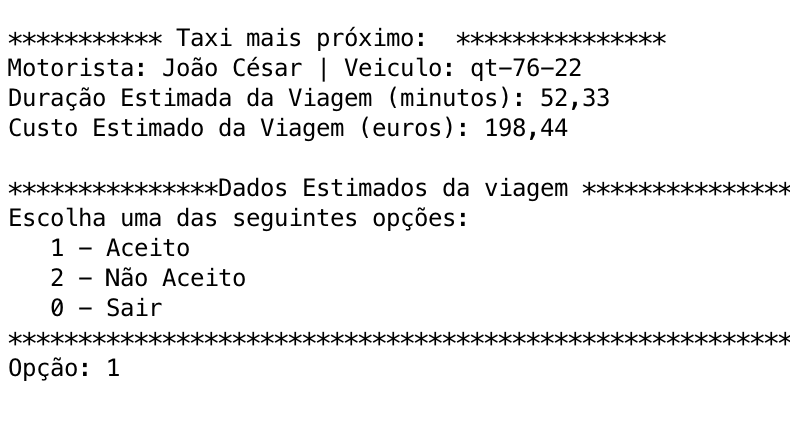
\includegraphics[scale=0.6]{imagem/taxiMaisProx}
	\caption{Menu com os dados do taxi mais próximo }
	\label{p3:fig:p3_taxiMaisProx}
\end{figure}

Se aceitar fazer a viagem aparecer-lhe-á o seguinte menu, com a informação do tempo que o táxi demorará até chegar à localização do cliente. 

\begin{figure}[htpb]
	\centering
	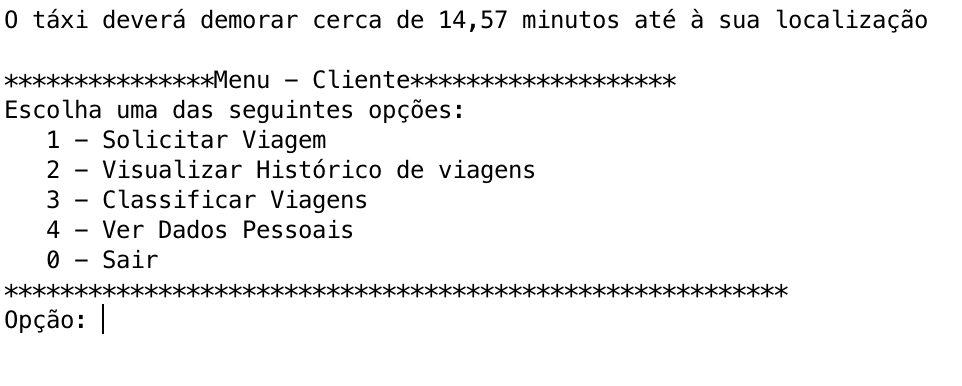
\includegraphics[scale=0.6]{imagem/aceitarViagem}
	\caption{Menu de Viagem aceite }
	\label{p3:fig:p3_aceitarViagem}
\end{figure}

Caso o cliente tenha efetuado uma viagem e esta ainda estiver a decorer, não poderá solicitar outra viagem sem que a atual tenha terminado. Será mostrada uma mensagem como a seguinte: 
\begin{figure}[htpb]
	\centering
	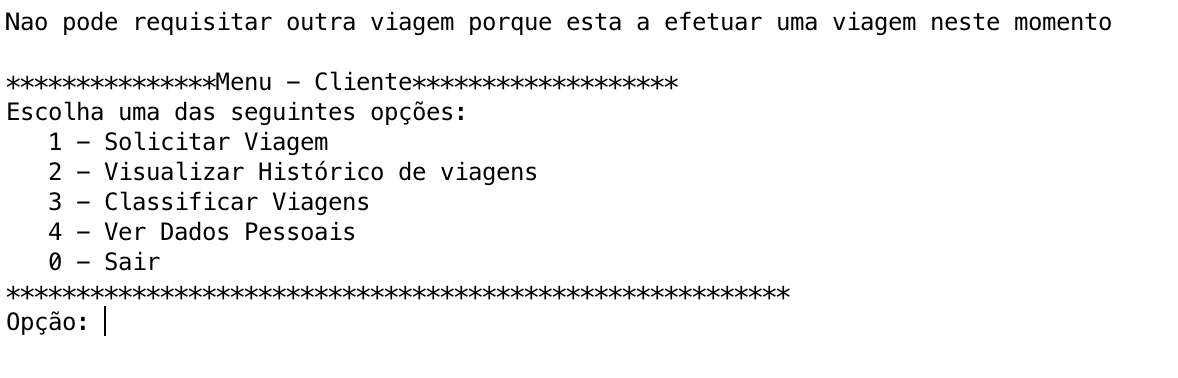
\includegraphics[scale=0.6]{imagem/erroEmViagem}
	\caption{Menu de Erro: Cliente está em viagem }
	\label{p3:fig:p3_erroEmViagem}
\end{figure}

É oferecida aos Clientes e a todos os outros utilizadores a possibilidade de verem os seus dados e editarem todos os campos com a excepção do email. 
\begin{figure}[htpb]
	\centering
	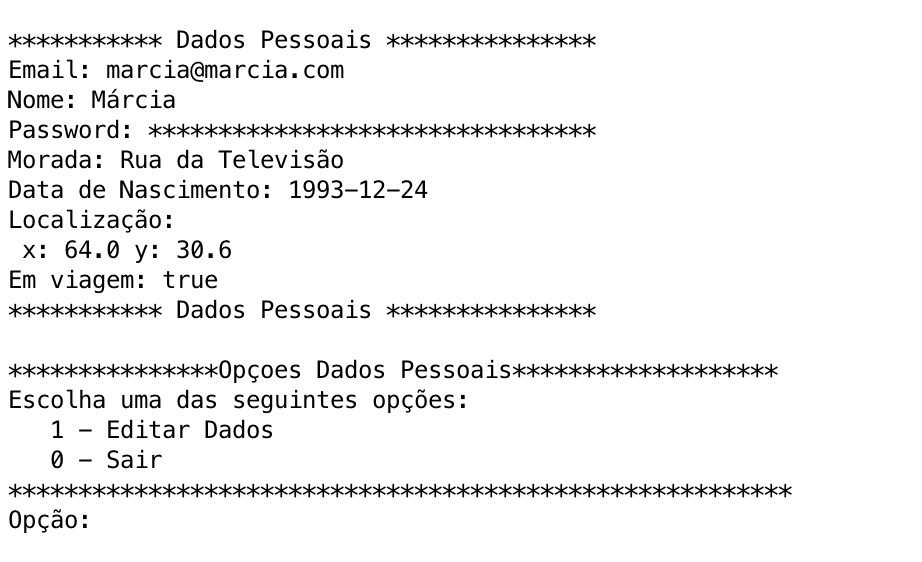
\includegraphics[scale=0.6]{imagem/verDadosPessoais}
	\caption{Menu de visualização e edição dos dados Pessoais }
	\label{p3:fig:p3_verDadosPessoais}
\end{figure}

\subsubsection{Motorista}
O motorista na UMeR poderá registar e remover o seu veiculo, gerir viagens é para iniciar uma viagem que esteja pendente; gerir horário de trabalho serve para não aceitar viagens quando não está a trabalhar. Poderá ver o histórico das viagens efetuadas, quais os seus melhores 10 clientes e ver e editar os seus dados pessoais. O menu apresentado será o seguinte: 
\begin{figure}[htpb]
	\centering
	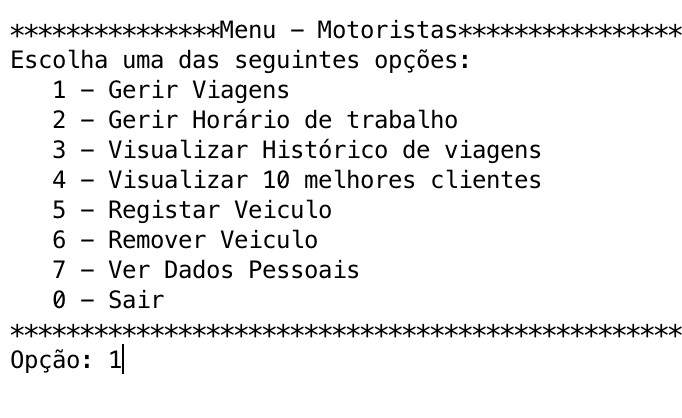
\includegraphics[scale=0.6]{imagem/menuMotorista}
	\caption{Menu de Motorista }
	\label{p3:fig:p3_menuMotorista}
\end{figure}

Após escolher gerir uma viagem será apresentado o menu com a opção de terminar viagem. Ao efetuar este passo a viagem passa a estar disponivel no histórico quer no cliente quer no motorista. 

\hfill
\noindent\begin{minipage}[b]{.4\textwidth}
	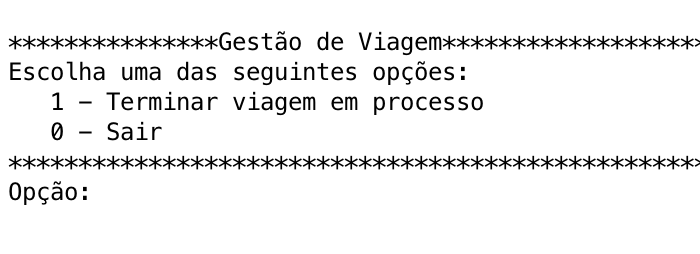
\includegraphics[scale=0.55]{imagem/gerirViagem}
	\small{Menu do motorista para terminar uma viagem}
\end{minipage} 
\hfill
\begin{minipage}[b]{.4\textwidth}
	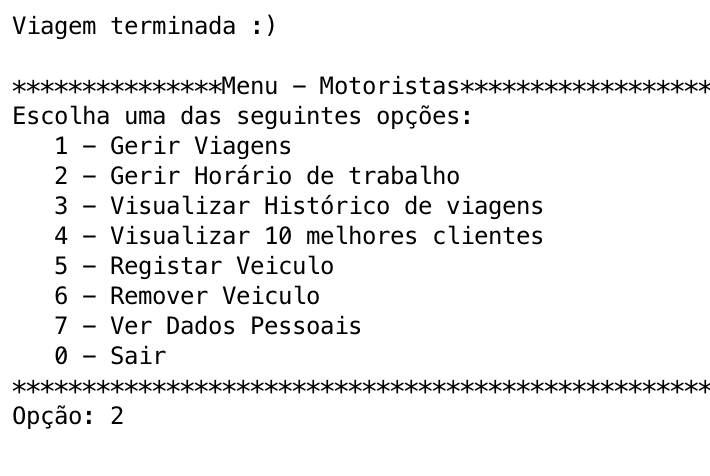
\includegraphics[scale=0.5]{imagem/viagemTerminada}
	\small{Menu após terminar viagem}
\end{minipage}
\hfill 

Na opção de gerir horário de trabalho é apresentado o seguinte menu em que o motorista o poderá terminar. 

\noindent\begin{minipage}[b]{.4\textwidth}
	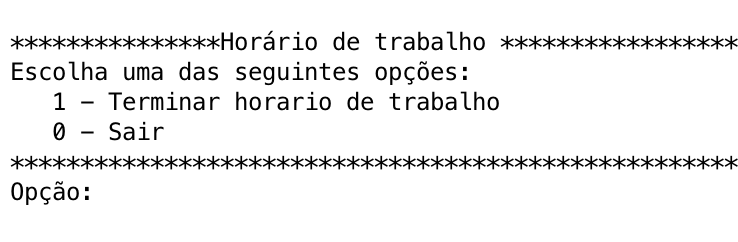
\includegraphics[scale=0.55]{imagem/gerirHorarioTrabalho}
	\small{Menu do motorista para iniciar horario de trabalho}
\end{minipage} 
\hfill
\begin{minipage}[b]{.4\textwidth}
	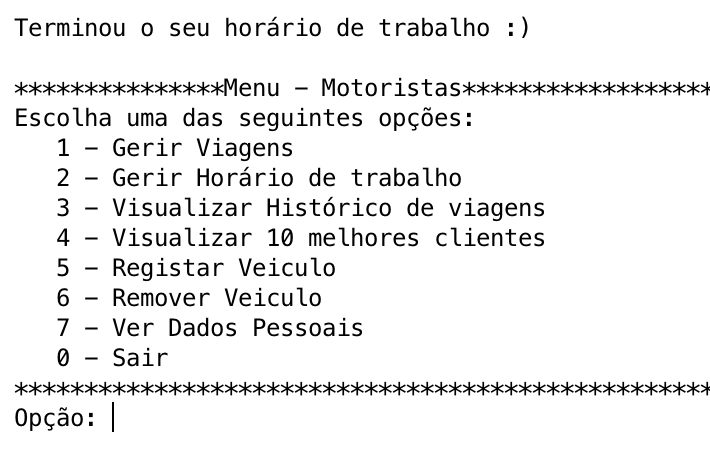
\includegraphics[scale=0.5]{imagem/terminouHorarioTrabalho}
	\small{Menu após terminar horário}
\end{minipage}
\hfill

Após terminar o horário, os menus mudam de modo a que o motorista possa voltar ao trabalho, sendo criados para tal os seguintes menus: 

\noindent\begin{minipage}[b]{.4\textwidth}
	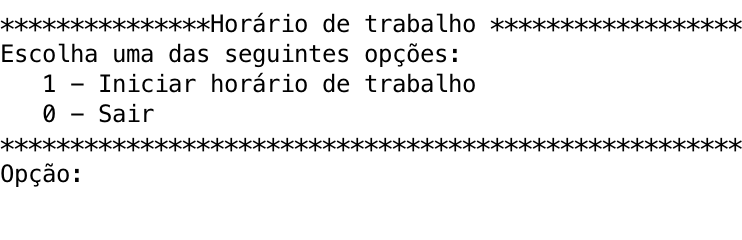
\includegraphics[scale=0.55]{imagem/iniciarHorarioTrabalho}
	\small{Menu do motorista para terminar horario de trabalho}
\end{minipage} 
\hfill
\begin{minipage}[b]{.4\textwidth}
	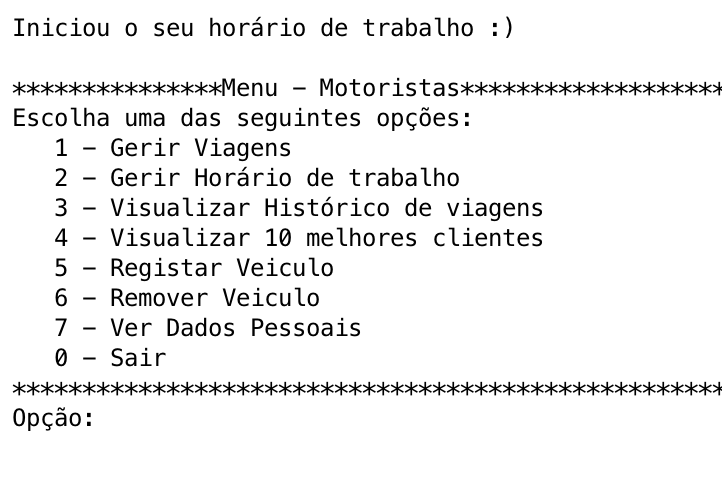
\includegraphics[scale=0.5]{imagem/iniciouHorarioTrabalho}
	\small{Menu após iniciar horário de trabalho}
\end{minipage}
\hfill



\begin{figure}[htpb]
	\centering
	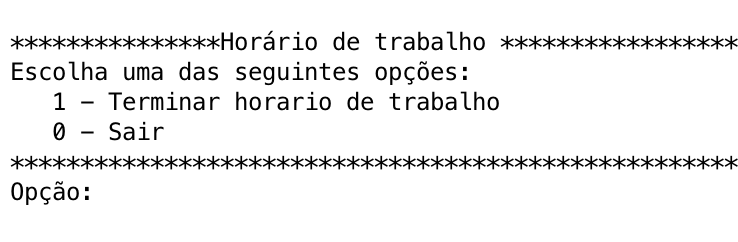
\includegraphics[scale=0.6]{imagem/gerirHorarioTrabalho}
	\caption{Menu de Motorista }
	\label{p3:fig:p3_gerirHorarioTrabalho}
\end{figure}

